% intro.tex
%
% Purpose:
%   Introduce the motivation, scope, and literature position of the report.
%
% Main algorithm:
%   This section describes the high-level combination of BIE, Rayleigh traces,
%   Bloch-mode selection, and center-cell matching.  It contains no executable
%   numerical algorithm.
%
% Based on:
%   pre/pre1/pre1.tex and the formulation notes in notes/theory/.
%
% Main changes:
%   The presentation is rewritten as a technical report introduction rather than
%   slide bullets.
%
% Numerical goal:
%   Clarify what the current formulation is meant to compute and how it relates
%   to existing periodic-waveguide methods.

\section{Introduction}

The goal of this report is to document the current numerical formulation for
periodic waveguide and line-defect computations in this repository.  The target
models are scalar Helmholtz transmission problems in geometries that are
quasiperiodic in the transverse variable \(y\) and open or periodic in the
longitudinal variable \(x\).  The central computational tasks are forced
lead-scattering problems and homogeneous eigenvalue or transmission-eigenvalue
searches.

The formulation is constructive and finite-dimensional.  It uses boundary
integral equations on material interfaces, compact artificial ports
\(\Gamma_-\) and \(\Gamma_+\), Rayleigh coordinates for Cauchy traces on those
ports, one-cell scattering matrices in the periodic half-leads, Bloch-mode
selection of incoming and outgoing trace subspaces, and a center-cell matching
system.  At the level of implementation, the half-leads are not represented by a
full infinite-dimensional exterior operator.  Instead, their effect is enforced
by requiring the port Cauchy trace to lie in a selected admissible subspace.

This distinction is important.  The Rayleigh basis is a coordinate basis on a
vertical wall; it is not itself the physical Bloch-mode basis of a periodic
lead.  Bloch modes are obtained from a one-cell propagation or scattering
problem, and only after applying a radiation or admissibility selection do they
define the physical incoming and outgoing trace spaces.  Once such a subspace is
selected, any well-conditioned basis of the same subspace may be used in the
global linear system.

\subsection{Geometry and notation}

The longitudinal lead direction is \(x\).  The transverse quasiperiodic
direction is \(y\), with period \(d\).  The three reference cells nearest the
defect are denoted
\[
  \Ccell^-,
  \qquad
  \Ccell^0,
  \qquad
  \Ccell^+ .
\]
The center obstacle is \(\Omega_0\), with boundary
\[
  \Sigma=\partial\Omega_0 .
\]
The left and right lead obstacles are denoted \(\Omega_-\) and \(\Omega_+\).
The artificial center-cell ports are
\[
  \Gamma_-=\{x=X_-\},
  \qquad
  \Gamma_+=\{x=X_+\}.
\]
The port normals are always the outward normals of the center cell:
\[
  \nu_{\Gamma_-}=-e_x,
  \qquad
  \nu_{\Gamma_+}=+e_x .
\]
When longitudinal periods of the negative and positive leads are needed, they
are written \(L_-\) and \(L_+\).  The symbol \(d\), not \(L\), is reserved for
the transverse period.

\begin{figure}[ht]
\centering
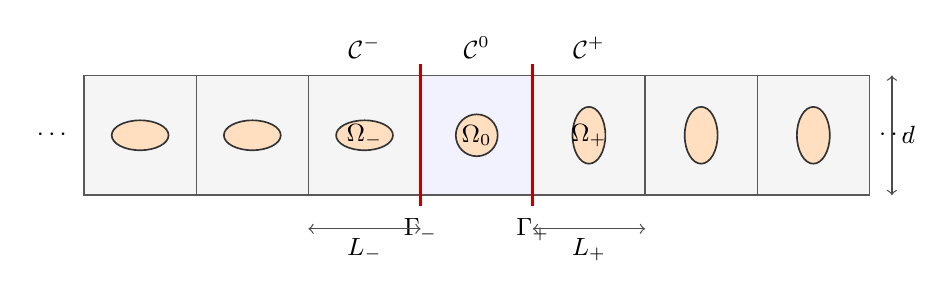
\begin{tikzpicture}[
  x=0.95cm,
  y=0.95cm,
  every node/.style={font=\small},
  cell/.style={draw=black!65, line width=0.5pt},
  leadcell/.style={fill=gray!8},
  centercell/.style={fill=blue!5},
  inclusion/.style={draw=black!80, fill=orange!25, line width=0.6pt},
  port/.style={draw=red!75!black, line width=1.1pt},
  dim/.style={<->, draw=black!70, line width=0.45pt}
]
  \foreach \x in {-5.25,-3.75,-2.25} {
    \draw[cell, leadcell] (\x,-0.8) rectangle ++(1.5,1.6);
    \draw[inclusion] (\x+0.75,0) ellipse [x radius=0.38, y radius=0.20];
  }

  \draw[cell, centercell] (-0.75,-0.8) rectangle (0.75,0.8);
  \draw[inclusion] (0,0) circle [radius=0.28];

  \foreach \x in {0.75,2.25,3.75} {
    \draw[cell, leadcell] (\x,-0.8) rectangle ++(1.5,1.6);
    \draw[inclusion] (\x+0.75,0) ellipse [x radius=0.22, y radius=0.38];
  }

  \draw[port] (-0.75,-0.95) -- (-0.75,0.95);
  \draw[port] (0.75,-0.95) -- (0.75,0.95);

  \node[above] at (-1.5,0.9) {$\mathcal C^-$};
  \node[above] at (0,0.9) {$\mathcal C^0$};
  \node[above] at (1.5,0.9) {$\mathcal C^+$};

  \node[below] at (-0.75,-0.98) {$\Gamma_-$};
  \node[below] at (0.75,-0.98) {$\Gamma_+$};

  \node at (-1.5,0) {$\Omega_-$};
  \node at (0,0) {$\Omega_0$};
  \node at (1.5,0) {$\Omega_+$};

  \draw[dim] (-2.25,-1.25) -- (-0.75,-1.25);
  \node[below] at (-1.5,-1.25) {$L_-$};
  \draw[dim] (0.75,-1.25) -- (2.25,-1.25);
  \node[below] at (1.5,-1.25) {$L_+$};

  \draw[dim] (5.55,-0.8) -- (5.55,0.8);
  \node[right] at (5.55,0) {$d$};
  \node[left] at (-5.35,0) {$\cdots$};
  \node[right] at (5.25,0) {$\cdots$};
\end{tikzpicture}
\caption{Schematic of the center cell, adjacent periodic lead cells, and compact
ports.  The diagram is only notational; the actual inclusion shapes are supplied
by the geometry routines.}
\label{fig:cells}
\end{figure}

\subsection{Relation to existing methods}

Boundary integral methods for quasiperiodic band-structure calculations are
closely related to the framework of Barnett and Greengard
\cite{BarnettGreengard2010}, including the numerical issues caused by
quasiperiodic Green functions and empty-cell resonances.  Exact boundary
conditions for locally perturbed periodic waveguides are treated in the work of
Joly, Li, and Fliss \cite{JolyLiFliss2006}, where half-guide exterior conditions
are expressed through periodic-guide Dirichlet-to-Neumann and related operators.
Coatl\'even \cite{Coatleven2012} treats a line-defect Helmholtz problem by
combining the Floquet--Bloch transform, Lippmann--Schwinger ideas, and
Dirichlet-to-Neumann maps.

The present formulation should be read as a finite-dimensional, compact-port
realization tailored to the current line-defect geometry.  It is not a
replacement for the full functional-analytic Dirichlet-to-Neumann theory.
Rather, it uses Rayleigh wall coordinates and one-cell Bloch/scattering
computations to build the admissible Cauchy trace subspaces used by the center
matching system.  This gives a practical route to matrix assembly, singular-value
scans, and convergence diagnostics while keeping the mathematical distinction
between rigorous exterior conditions and numerical truncations visible.
